%!TEX root = Main.tex
% Project analysis: words
\chapter{Project Analysis and Reflection} % (fold)
\label{cha:project_analysis}

This chapter presents an analysis of the final solution, evaluating its primary strengths and weaknesses.  An overview and reflection of the project management is then given.

\section{Analysis of Solution} % (fold)
\label{sec:analysis_of_solution}

	\subsection{The FPGA} % (fold)
	\label{sub:analysis_the_fpga}
		The FPGA used was very small, and the full required design could not fit on it.  In particular, the size of the model had to be reduced, so that each Gaussian mean and variance had fewer than 25 components, and not all 7000 senones were processed.  However, what has been implemented is adequate to prove the concept, and demonstrate the advantages gained from using an FPGA.  In addition, it was known from the start that the full model would never fit, and so although this is a practical limitation, it does not make the project less worthwhile.

		In the previous chapter, various benchmarks were presented in the form of timing data.  It was shown that the FPGA was capable of calculating senone scores far faster than the traditional processor, albeit with a loss of accuracy.  This is similar to results achieved by Melnikoff \cite{melnikoff2003speech} and Speech Silicon \cite{schuster2006speech}, and supports the principle that custom made hardware is faster than general purpose processors.  For real-time speech recognition, getting the senone scores as fast as possible is very important, as it allows more time for decoding tasks.  Thus, using an FPGA may be beneficial, especially in embedded systems.  It is possible to extrapolate, from the data gathered, the system speed when a larger model is implemented.  If the full model (7000 senones, 25 components) was used, the scores would be computed in about 3.5ms, leaving 6.5ms (of a 10ms window) for pre-processing and decoding (this excludes communications time).

		A big disadvantage of using an FPGA, in such a system, is the need to communicate to it.  The communication is an added step that adds time to the senone scoring process, and, if it is not fast enough, may render the use of an FPGA not worthwhile.  The implemented communication method (UART) is extremely slow and is the weakest point of the system.  It was used primarily for the ease of implementation, and because at this stage real-time operations are not required.  However, for this system to be realistically useful, a better communication method needs to be developed -- either a far faster serial bus or some form of hybrid serial-parallel connection.

		% Additionally, the number format used caused the calculation accuracy to be reduced
	% subsection the_fpga (end)

	% Evaluate the speed - how long did each cycle take.  How much time was added by adding another component? or another senone? Extrapolate?

	\subsection{The processor} % (fold)
	\label{sub:analysis_the_processor}
		The biggest problem, or limitation, with the current preprocessing system is the MFCC calculation step.  An external library was used, due to time contraints, that was not optimised for the project's requirements at all.  The HTK has a far faster implementation of this step, 

		However, what has been implemented is a good demonstration of the capabilities of this processor.
	% subsection the_processor (end)


	\subsection{Complete system} % (fold)
	\label{sub:complete_system_analysis}
		TODO?
	% subsection complete_system_analysis (end)
% section analysis_of_solution (end)


\section{Deviations From Original Goals} % (fold)
\label{sec:deviations_from_original_goals}
	Originally, while planning the project, the goal had been to implement a complete speech recognition system, from pre-processing to Viterbi decoding.  However, as more was learnt about the systems involved, it became clear that it was far to large a subject to attack in a single project.  Thus, the biggest change from initial plans was to narrow the project's focus down to a particular area of speech recognition.  However, with respect to the focussed goal, the results achieved are very satisfactoy.

	Development began by following the Gantt chart shown in Figure~\ref{fig:gantt1}, which was also presented in the project Interim Report.  However, building a software decoder proved to be far more time consuming than expected.  At this point, the decision was made to change the focus, as mentioned above.  The majority of the design and implementation was then completed before April, as in the Gantt chart.

	\begin{figure}[tb]
		\begin{center}
			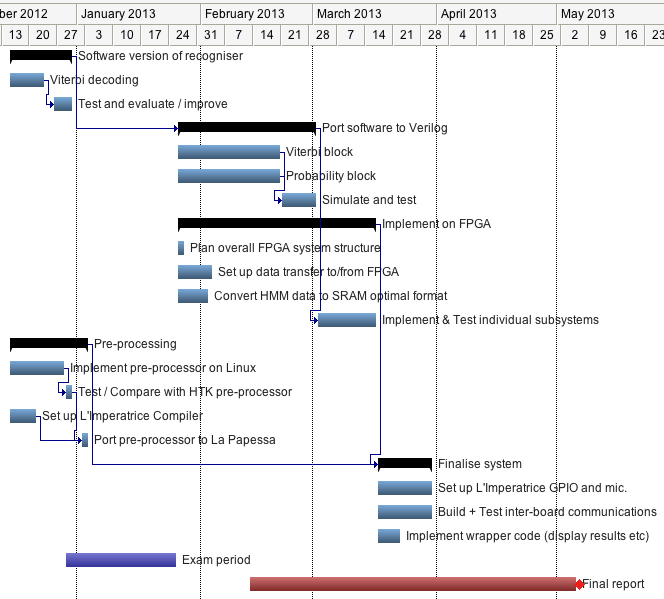
\includegraphics[width=1.1\textwidth,angle=90]{gantt-chart-interim.png}
		\end{center}
		\caption{Interim Gantt chart for remaining work}
		\label{fig:gantt2}
	\end{figure}
% section deviations_from_original_goals (end)


\section{Contingency Planning} % (fold)
\label{sec:contingency_planning}
% section contingency_planning (end)
	Efforts were made to divide the project work up into sections that were independent.  If at all possible, it was modularised, so that if one section became unfeasible, it could be dropped without affecting the outcome of the final product greatly.  This indeed happened with the Viterbi decoding, which was dropped without affecting the other parts.  The Micro Arcana especially, was completely unknown, and therefore several alternatives were lined up in case it became impossible to use it.

	A variety of measures were taken in order to protect against the possibility of work being lost.  Primarily, the source code and designs were backed up on external storage, as well as being regularly uploaded to a Github repository.  The `Git' version control software was used throughout the project.  The primary benefit was that it enforced a regular process of adding changes, validating them, and committing them to the repository.  This helps keep development on-track and focussed, as well as preserving sets of code that work.  It also provides a logbook style commit history, which allowed the progress of the project to be observed.
% chapter project_analysis (end)